%!TEX root = project.tex

\chapter*{About this project}
\paragraph{Abstract}
A dynamic web app that creates curated playlists based on multiple user's music preferences using Spotify. Built with React, Flask, Python, Node.js, Mocha, AWS and Mongo.

\paragraph{Authors}
\begin{flushleft}
	Eddie Eldridge
	
	Danielis Joniskis
	
	Keith Higgins
	
	Three students from the Galway-Mayo Institute of Technology
\end{flushleft}



\chapter{Introduction}
The introduction should be about three to five pages long.
Make sure you use references~\cite{einstein}
\begin{flushleft}
	Context for the Project.
	
	
	Objectives of the Project.
	
	
	Is the reader 100 percent of what the project is all about 
\end{flushleft}


\chapter{Context}
\begin{itemize}
\item Provide a context for your project.
\item Set out the objectives of the project
\item Briefly list each chapter / section and provide a 1-2 line description of what each section contains.
\item List the resource URL (GitHub address) for the project and provide a brief list of the main elements at the URL.
\end{itemize}

\section{Filler}
Lorem ipsum dolor sit amet, consectetur adipiscing elit. Etiam mi enim, interdum ut elit lobortis, bibendum tempus diam. Etiam turpis ex, viverra tristique finibus nec, feugiat at metus. Curabitur tempus gravida interdum. Donec ac felis a lorem scelerisque elementum. Vestibulum sit amet gravida tortor, a iaculis orci. Nam a molestie augue. Curabitur malesuada odio at mattis molestie. In hac habitasse platea dictumst. Donec eu lectus eget risus hendrerit euismod nec at orci. Praesent porttitor aliquam diam, eu vestibulum nisl sollicitudin vel. Nullam sed egestas mi.

Quisque vel erat a justo volutpat auctor a nec odio. Sed rhoncus augue sit amet nisl tincidunt, vitae cursus tellus efficitur. Class aptent taciti sociosqu ad litora torquent per conubia nostra, per inceptos himenaeos. Pellentesque et auctor dui. Fusce ornare odio ipsum, et laoreet mi molestie sed. Cras at massa sit amet ipsum gravida aliquam. Nulla suscipit porta imperdiet. Fusce eros neque, bibendum sit amet consequat non, pulvinar quis ipsum.

\subsection{More filler}
Donec fermentum sapien ac rhoncus egestas. Nullam condimentum condimentum eros sit amet semper. Nam maximus condimentum ligula. Praesent faucibus in nisi vitae tempus. Sed pellentesque eleifend ante, ac malesuada nibh dapibus nec. Phasellus nisi erat, pulvinar vel sagittis sed, auctor et magna. Quisque finibus augue elit, consequat dignissim purus mollis nec. Duis ultricies euismod tortor, nec sodales libero pellentesque et. Interdum et malesuada fames ac ante ipsum primis in faucibus.

Donec id interdum felis, in semper lacus. Mauris volutpat justo at ex dignissim, sit amet viverra massa pellentesque. Suspendisse potenti. Praesent sit amet ipsum non nibh eleifend pretium. In pretium sapien quam, nec pretium leo consequat nec. Pellentesque non dui lacus. Aenean sed massa lacinia, vehicula ante et, sagittis leo. Sed nec nisl ac tellus scelerisque consequat. Ut arcu metus, eleifend rhoncus sapien sed, consequat tincidunt erat. Cras ut vulputate ipsum.

Curabitur et efficitur augue. Proin condimentum ultrices facilisis. Mauris nisi ante, ultrices sed libero eget, ultrices malesuada augue. Morbi libero magna, faucibus in nunc vitae, ultricies efficitur nisl. Donec eleifend elementum massa, sed eleifend velit aliquet gravida. In ac mattis est, quis sodales neque. Etiam finibus quis tortor eu consequat. Nullam condimentum est eget pulvinar ultricies. Suspendisse ut maximus quam, sed rhoncus urna.

\section{Filler}
Phasellus eu tellus tristique nulla porttitor convallis. Vestibulum ac est eget diam mollis consectetur. Donec egestas facilisis consectetur. Donec magna orci, dignissim vel sem quis, efficitur condimentum felis. Donec mollis leo a nulla imperdiet, in bibendum augue varius. Quisque molestie massa enim, vitae ornare lacus imperdiet non. Donec et ipsum id ante imperdiet mollis. Nullam est est, euismod sit amet cursus a, feugiat a lectus. Integer sed mauris dolor.

Mauris blandit neque tortor, consequat aliquam nisi aliquam vitae. Integer urna dolor, fermentum ut iaculis ut, semper eu lacus. Curabitur mollis at lectus at venenatis. Donec fringilla diam ac risus imperdiet suscipit. Aliquam convallis quam vitae turpis interdum, quis pharetra lacus tincidunt. Nam dictum maximus lectus, vitae faucibus ante. Morbi accumsan velit nec massa tincidunt porttitor. Nullam gravida at justo id viverra. Mauris ante nulla, eleifend vitae sem vitae, porttitor lobortis eros.

Cras tincidunt elit id nisi aliquam, id convallis ex bibendum. Sed vel odio fringilla, congue leo quis, aliquam metus. Nunc tempor vehicula lorem eu ultrices. Curabitur at libero luctus, gravida lectus sed, viverra mi. Cras ultrices aliquet elementum. Pellentesque habitant morbi tristique senectus et netus et malesuada fames ac turpis egestas. Sed metus ante, suscipit sit amet finibus ut, gravida et orci. Nunc est odio, luctus quis diam in, porta molestie magna. Interdum et malesuada fames ac ante ipsum primis in faucibus. Mauris pulvinar lacus odio, luctus tincidunt magna auctor ut. Ut fermentum nisl rhoncus, tempus nulla eget, faucibus tortor. Suspendisse eu ex nec nunc mollis pulvinar. Nunc luctus tempus tellus eleifend porta. Nulla scelerisque porttitor turpis porttitor mollis.

Duis elementum efficitur auctor. Nam nisi nulla, fermentum sed arcu vel, posuere semper dui. Fusce ac imperdiet felis. Aenean quis vestibulum nisl. Integer sit amet tristique neque, at suscipit tortor. Morbi et placerat ante, vel molestie dui. Vivamus in nibh eget massa facilisis accumsan. Nunc et purus ac urna fermentum ultrices eget sit amet justo. Class aptent taciti sociosqu ad litora torquent per conubia nostra, per inceptos himenaeos. Cras elementum dui nunc, ac tempor odio semper et. Ut est ipsum, sollicitudin eleifend nisl eu, scelerisque cursus nunc. Nam at lectus vulputate, volutpat tellus vel, pharetra mauris. Integer at aliquam massa, at iaculis sem. Morbi nec imperdiet odio. In hac habitasse platea dictumst.

Mauris a neque lobortis, venenatis erat ut, eleifend quam. Nullam tincidunt tellus quis ligula bibendum, a malesuada erat gravida. Phasellus eget tellus non risus tincidunt sagittis condimentum quis enim. Donec feugiat sapien sit amet tincidunt fringilla. Vivamus in urna accumsan, vehicula sem in, sodales mauris. Aenean odio eros, tristique non varius id, tincidunt et neque. Maecenas tempor, ipsum et sollicitudin rhoncus, nibh eros tempus dolor, vitae dictum justo massa in eros. Proin nec lorem urna. In ullamcorper vitae felis sit amet tincidunt. Maecenas consectetur iaculis est, eu finibus mi scelerisque et. Nulla id ex varius, ultrices eros nec, luctus est. Aenean ac ex eget dui pretium mattis. Ut vitae nunc lectus. Proin suscipit risus eget ligula sollicitudin vulputate et id lectus.


\chapter{Methodology}
About one to two pages.
Describe the way you went about your project:
\begin{itemize}
\item Agile / incremental and iterative approach to development. Planning, meetings.
\item What about validation and testing? Junit or some other framework.
\item If team based, did you use GitHub during the development process.
\item Selection criteria for algorithms, languages, platforms and technolo-gies.
\end{itemize}
Check out the nice graphs in Figure \ref{tikz:graphs}, and the nice diagram in Figure \ref{tikz:mydiagram}.

\begin{figure}
  \centering
  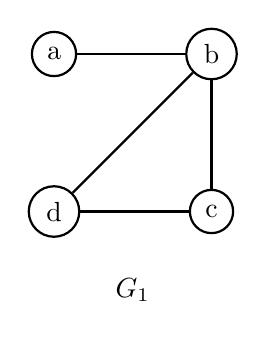
\begin{tikzpicture}
  \begin{scope}[every node/.style={circle,thick,draw}]
  \node (a) at (0,2) {a};
  \node (b) at (2,2) {b};
  \node (c) at (2,0) {c};
  \node (d) at (0,0) {d};
  \end{scope}
  \begin{scope}[every edge/.style={draw=black,thick}]
  \path (a) edge (b);
  \path (b) edge (c);
  \path (b) edge (d);
  \path (c) edge (d);
  \end{scope}
  \node () at (1,-1) {$G_1$};
  \end{tikzpicture}
  \hspace{1.5cm}
  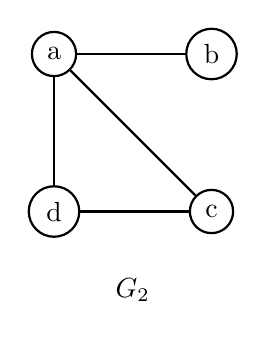
\begin{tikzpicture}
  \begin{scope}[every node/.style={circle,thick,draw}]
  \node (1) at (0,2) {a};
  \node (2) at (2,2) {b};
  \node (3) at (2,0) {c};
  \node (4) at (0,0) {d};
  \end{scope}
  \begin{scope}[every edge/.style={draw=black,thick}]
  \path (1) edge (2);
  \path (1) edge (3);
  \path (1) edge (4);
  \path (3) edge (4);
  \end{scope}
  \node () at (1,-1) {$G_2$};
  \end{tikzpicture}
  \caption{Nice pictures}
  \label{tikz:graphs}
\end{figure}


\begin{figure}
  \centering
  \begin{tikzpicture}[node distance=6cm]
  \node (a) [rect] {A Big Blue Block};
  \node (b) [oval, right of=a] {And His Oval Friend};
  \draw [line] (a) -- (b);
  \end{tikzpicture}
  \caption{Nice pictures}
  \label{tikz:graphs}
\end{figure}


\chapter{Technology Review}
About seven to ten pages.
\begin{itemize}
\item Describe each of the technologies you used at a conceptual level. Standards, Database Model (e.g. MongoDB, CouchDB), XMl, WSDL, JSON, JAXP.
\item Use references (IEEE format, e.g. [1]), Books, Papers, URLs (timestamp) – sources should be authoritative. 
\end{itemize}

\section{AWS}
Amazon Web Services offers reliable, scalable, and inexpensive cloud computing services.

\begin{minted}{xml}
<this>
  <looks lookswhat="good">
    Good
  </looks>
</this>
\end{minted}

\section{MongoDB}
MongoDB is an open-source, document database designed for ease of development and scaling. MongoDB stores data in JSON-like documents, which makes the database very flexible and scalable.\cite{w3schools}

\section{Flask}
Flask is a microframework for Python.

\section{Python}
Python is a programming language that lets you work more quickly and integrate your systems more effectively.

\section{Mocha}
Mocha is a JavaScript test framework running on Node.js. Mocha tests run serially, allowing for flexible and accurate reporting

\section{React}
React is a JavaScript library for building user interfaces. React is developed by Facebook. It is a tool for building UI components. React uses Babel to convert JSX (JavaScript XML) into JavaScript. Babel is a JavaScript compiler that can translate markup or programming languages into JavaScript. With Babel, you can use the newest features of JavaScript (ES6 - ECMAScript 2015). \cite{w3schools}

\chapter{System Design}
As many pages as needed.
\begin{itemize}
\item Architecture, UML etc. An overview of the different components of the system. Diagrams etc… Screen shots etc.
\end{itemize}

\begin{table}[h]
  \centering
  \begin{tabular}{x{2cm}p{3cm}}
    \toprule \\
    Column 1 & Column 2 \\
    \midrule \\
    Rows 2.1 & Row 2.2 \\
    \bottomrule
  \end{tabular}
  \caption{A table.}
  \label{table:mytable}
\end{table}

\chapter{System Evaluation}
As many pages as needed.
\begin{itemize}
\item Prove that your software is robust. How? Testing etc. 
\item Use performance benchmarks (space and time) if algorithmic.
\item Measure the outcomes / outputs of your system / software against the objectives from the Introduction.
\item Highlight any limitations or opportuni-ties in your approach or technologies used.
\end{itemize}

\chapter{Conclusion}
About three pages.

\begin{itemize}
\item Briefly summarise your context and ob-jectives (a few lines).
\item Highlight your findings from the evalua-tion section / chapter and any opportuni-ties identified.
\end{itemize}

